%% it_the_state_of_art.tex
%% $Id: it_the_state_of_art.tex 61 2012-05-03 13:58:03Z bless $
%%

\chapter{Methodik und Material}
\label{ch:ITStateOfArt}
%% ==============================

Das Kapitel „Methodik und Material“ befasst sich mit dem Vorgehen bzw. dem Aufbau der Bachelor-Thesis. Es soll weiterhin auf die zur Klärung der Leitfrage notwendigen Materialen hingeweisen und kurz eingegangen werden.

%% ==============================
\section{Vorgehensweise der Untersuchung}
%% ==============================

Die nachfolgende, selbsterstellte Grafik ist eine abstrakte Abbildung der Struktur zur Vorgehensweise in dieser Arbeit.

\begin{figure}[H]
 \centering
 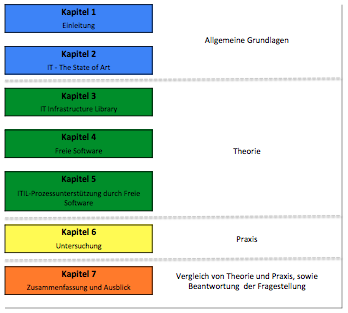
\includegraphics[scale=0.7]{images/Struktur_der_BA_v2.png}
 \caption{Struktur der Arbeit}
 \label{fig:Struktur_BA}
\end{figure}

Zu Beginn wird durch die Gesamtbetrachtung und durch das Aufzeigen des IST-Stands der derzeitigen IT die Aktualität und Bedeutung des Themas gefestigt.
Das Kapitel „IT - The State of Art“ gibt Aufschluss über den aktuellen Einsatzgrad von ITIL in IT-Unternehmen und soll auf etwaige daraus ableitbare Handlungspotentiale hinweisen. \\
Hier wird das Thema IT Service Managementprozesse hervorgehoben beleuchtet, da dort der Ansatz für den Einsatz von unterstützender „Freier“ Software zu finden ist.\\
Weiterführend wird auf den Aufbau und den Inhalt, sowie auf die Anwendbarkeit und die Einsatzmöglichkeiten des ITIL-Referenzmodells eingegangen und an Hand der Literatur beschreiben. 
\\
Hinzu kommt die Definition „Freier“ Software, die dem Leser ein grundsätzliches Verständnis über bestehende „Freie“ Softwareprodukte vermittelt. Hier liegt das Hauptaugenmerk auf speziell für ITIL zugeschnittene Software.\\
Unterstützend dazu beschreibt ein weiteres Kapitel die Rahmenbedingungen und Begleitaspekte einer ITIL-Prozessunterstützung durch „Freie“ Software.
\\
\\
Folgend auf die theoretischen Kapitel beschäftigt sich der empirische Teil mit Erfahrungen aus der Praxis.
Hierzu wird die Herangehensweise der Softwareauswahl beschrieben und an Hand einer eigens erstellten konzeptionellen Software-Architektur für die IT Service Managementprozesse das Einsatzgebiet der „Freien“ Software verdeutlicht.\\   
Der Vergleich zwischen Theorie und Praxis wird in weiterer Folge vollzogen und dem Leser in einer zusammenfassenden und übersichtlichen Form zur Verfügung gestellt.

%% ==============================
\section{Abgrenzung}
%% ==============================
\label{ch:ITStateOfArt:sec:Abgrenzung}

In der Bachelor Arbeit wird lediglich der Einsatz von „Freier“ Software mit der aktuellen Edition von ITIL, der ITIL 2011, bearbeitet. 
\\
Weiterhin wird auf Grund der Fülle an „Freier“ Software, die sich zur Zeit auf dem Markt befindet, auch hier nur ein bestimmter Teil zur Lösung der Problem- bzw. Leitfrage verwendet. Diese wird nach bestimmten Kriterien ausgewählt. Diese Kriterien liegen in den Bereichen Schnittstellenverfügbarkeit, Nutzbarkeit und vor allem der Sicherheit.\\
Auch die vollständige Implementierung der ausgewählten Software ist nicht Teil dieser Bachelor-Thesis. 

%% ==============================
\section{Erforderliches Material}
%% ==============================
\label{ch:ITStateOfArt:sec:ErforderlichesMaterial}

Wichtigstes Material zur Lösung der Hypothesen und Problemstellung ist vor allem die Literatur rund um ITIL 2011. Hierbei stechen 3 Werke besonders neben den Standardwerken der OGC heraus, die Folgend aufgeführt und kurz beschrieben werden:\\
\begin{description}
\item[IT Service Management]~\par
\end{description}
Das Buch „ITIL 2011 Edition - Das Taschenbuch“ \cite{ITGovITIL} von Van Haren Publishing bietet eine kurze Zusammenfassung von ITIL und stellt seine Prozesse kompakt dar. Es wurde vor allem für praktische Anwender mit ersten ITIL-Erfahrungen geschrieben. Es verschafft dem Leser einen guten Überblick über das Thema und eignet sich besonders gut als Nachschlagewerk. Weiterhin deckt dieses Buch die Anforderungs-Spezifikationen des ITIL-Foundation Lehrplans ab und kann deswegen auch als Teil der Vorbereitung für die ITIL-Foundation Zertifizierung verwendet werden.\\
\begin{description}
\item[IT Service Management in der Praxis]~\par
\end{description}Martin Beims erläutert in seinem Buch „IT-Service Management mit ITIL: ITIL Edition 2011, ISO20000:2011 und PRINCE in der Praxis“ \cite{BeimsITManage} sehr gut den Kontext zwischen dem ITIL-Referensmodell und dem pragmatischen Ansatz. Der Author untermauert diesen mit Studien, Praxisbeispielen und Erklärungen des ITIL-Standards. Weiter beleuchtet Beims auch die Wichtigkeit eines effizienten Projektmanagements, von Rollendefinitionen durch „Best Practices“. Abgerundet wird das alles durch die kurze Vorstellung von weiteren Standards und Zertifizierungsmöglichkeiten.\\
\begin{description}
\item[ITIL - Das ITSM Framework]~\par
\end{description}
Ebenso praxisnah wie Martin Beims bringt auch der Author Peter Köhler in seinem Buch „ITIL – Das IT-Servicemanagement Framework“ \cite{KoehlerITSM} das Thema ITIL und dessen pragmatischen Begleitaspekte auf einen gemeinsamen Punkt. Es werden grundsätzliche Begriffe erläutert, die das Umfeld um ITIL und ITSM beschrieben. Bei Einzelnen der fünf Hauptprozessen geht der Author zudem entsprechend in die Tiefe.

Weitere Literatur, zur Open-Source-Software und der Erstellung einer Software-Architektur, tragen ebenfalls zur Lösung bei und sind im Literaturverzeichnis vermerkt..
Neben der Literatur wurde auch eine SWOT-Analyse erstellt, wobei das dort notwendige Wissen auf dem Erlernten des Moduls „BWL“ des Studiengangs Wirtschaftsinformatik der Hochschule für Telekommunikation Leipzig beruht.


%%% Local Variables: 
%%% mode: latex
%%% TeX-master: "thesis"
%%% End: 
